\documentclass[a4paper,12pt]{article} % тип документа

% report, book

% Рисунки
\usepackage{graphicx}
\usepackage{wrapfig}
\usepackage{mathtext}
\usepackage[left=2cm,right=2cm,
    top=2cm,bottom=2cm,bindingoffset=0cm]{geometry}

\usepackage{hyperref}
\usepackage[rgb]{xcolor}
\hypersetup{				% Гиперссылки
    colorlinks=true,       	% false: ссылки в рамках
	urlcolor=blue          % на URL
}

%  Русский язык
\usepackage[T2A]{fontenc}			% кодировка
\usepackage[utf8]{inputenc}			% кодировка исходного текста
\usepackage[english,russian]{babel}	% локализация и переносы
\addto\captionsrussian{\def\refname{Список используемой литературы}}

% Математика
\usepackage{amsmath,amsfonts,amssymb,amsthm,mathtools} 
\usepackage{titlesec}
\titlelabel{\thetitle.\quad}

\usepackage{wasysym}

\date{}
\begin{document}

\begin{titlepage}

\thispagestyle{empty}

\centerline{МОСКОВСКИЙ ФИЗИКО-ТЕХНИЧЕСКИЙ ИНСТИТУТ}
\centerline{(НАЦИОНАЛЬНЫЙ ИССЛЕДОВАТЕЛЬСКИЙ УНИВЕРСИТЕТ)}

\vfill

\centerline{\huge{Лабораторная работа 3.5.1}}
\centerline{\large{по теме:}}
\centerline{\LARGE{<<Изучение плазмы газового разряда в неоне>>}}

\vfill

Студент группы Б02-109 \hfill Назарчук Анна

\vfill

\centerline{Долгопрудный, 2022}
\clearpage
\end{titlepage} 
\section{Аннотация}
В работе исследована плазма газового разряда в неоне с помощью двойного зонда. Экспериментально получена вольт-амперная характеристика разряда в режиме поднормального тлеющего разряда. Расчитаны зондовые характеристики, измерены основные параметры плазмы.


\section{Введение}
Как известно, вещество может находиться в трёх агрегатных состояниях
— твёрдом, жидком и газообразном, причём эти состояния последовательно
сменяются по мере возрастания температуры. Если и дальше
нагревать газ, то сначала молекулы диссоциируют на атомы, а затем и
атомы распадаются на электроны и ионы, так что газ становится ионизованным,
представляя собой смесь из свободных электронов и ионов,
а также нейтральных частиц. Такое состояние газа нельзя описывать как обычный газ с некоторыми частицами, требуются дополнительные параметры, описывающие движение такого газа (плазмы). Определение таких параметров, как тип разряда и других основных характеристик, и является целью данной работы.


\section{Методика измерений}

Для определения основных характеристик плазмы произведены измерения с помощью двойного зонда - системы, состоящей из двух одинаковых зондов на небольшом растоянии друг от друга, между которыми создается небольшая (по сравнению с потенциалом, до которого заряжается зонд, помещенный в плазму) разность потенциалов $U$. Теоретически получена зависимость тока от напряжения между зондами: (она также представлена на графике \ref{двойной}).\cite{labnik}
\begin{equation}
I = I_{iн} th\frac{eU}{2k_БT_e}
\end{equation}
\begin{figure}[h!]
\begin{center}
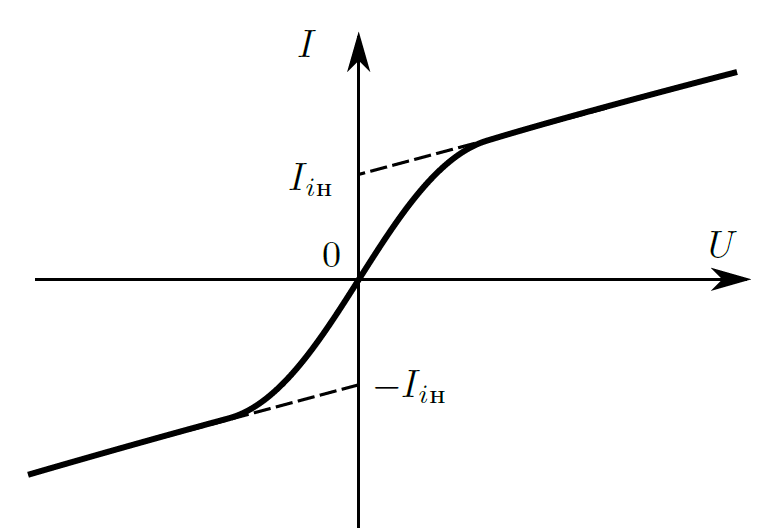
\includegraphics[width=0.6\textwidth]{Двойной}
\caption{Качественный вид экспериментальной вольт-амперной характеристики двойного зонда \cite{labnik}.} \label{двойной}
\end{center}
\end{figure}

При рассмотрении этой формулы вблизи $U = 0$:
\begin{equation}
\label{двойной_зонд}
k_БT_e = \frac{1}{2}\frac{eI_{iн}}{\frac{dI}{dU}|_{U=0}}
\end{equation}
Для определения температуры электронов в плазме из пересечения асимптот с осью $U=0$ найдена $I_{in}$ и вычислен наклон графика в начале координат. По этим известным параметрам определена концентрацию заряженных частиц, используя полуэмперическую формулу Д. Бома: \cite{labnik}
\begin{equation} 
\label{бом}
I_{iн} \approx 0.4 n_iS\sqrt{\frac{2k_БT_e}{m_i}}
\end{equation}
Основными характеристиками плазмы являются плазменная частота колебаний $\omega_p$ (определяет временной масштаб движения плазмы), дебаевский радиус $r_{De}$ (определяет пространственный масштаб явления в плазме), поляризационная длина $r_D$ (определяет масштаб, на котором можно считать плазму квазинейтральной), среднее число ионов в дебаевской сфере $N_D$ (при больших значениях плазма считается идеальной). Теоретические формулы для вычисление этих величин приведены в таблице \ref{формулы}.\cite{labnik}
\begin{table}[h!]
\caption{Теоретические выражения для основных характеристик плазмы}
\label{формулы}
\begin{tabular}{|l|l|}
\hline
Величина   & Теоретическое выражение                                 \\ \hline
$\omega_p$ & $\sqrt{\frac{4\pi n_e e^2}{m_e}}$                       \\ \hline
$r_{De} $  & $\sqrt{\frac{k_Б T_e}{4\pi n_e e^2}}$                   \\ \hline
$r_D $     & $\sqrt{\frac{k_Б}{4\pi n_e e^2}\frac{T_eT_i}{T_e+T_i}}$ \\ \hline
$N_D $     & $\frac{4}{3}\pi n_ir^3_D$                               \\ \hline
\end{tabular}
\end{table}

\section{Установка}
Схема экспериментальной установки приведена на рисунке \ref{установка}. Трубка наполнена изотопом неона $^{22}Ne$ при давлении 2 мм рт. ст. При подключении к высоковольтному источнику питания анода-I между ним и катодом возникает газовый разряд. Ток разряда измеряется миллиамперметром $A_1$, а падение
напряжения на разрядной трубке — вольтметром $V_1$. При подключении к высоковольтному источнику питания анода-II разряд возникает в пространстве между катодом и анодом-II, где находится двойной зонд, используемый
для диагностики плазмы положительного столба.

\begin{figure}[h!]
\begin{center}
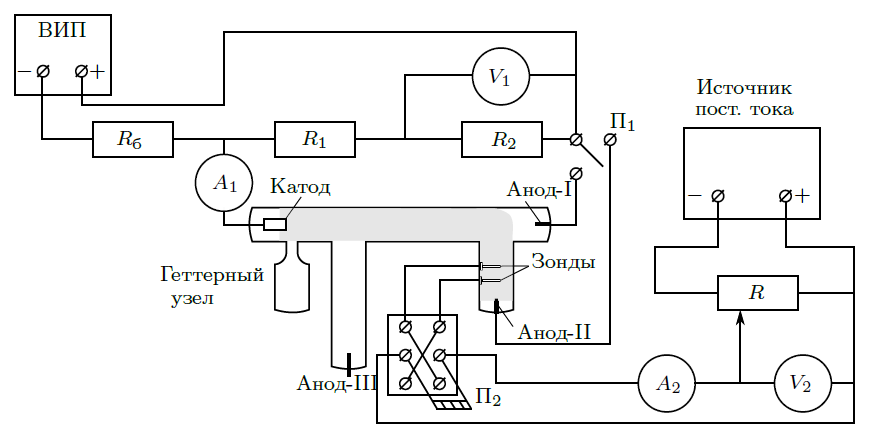
\includegraphics[width=0.6\textwidth]{Установка}
\caption{Схема экспериментальной установки для исследования газового разряда при давлениях $\sim $2 Торр. $R_б$ - балластный резистор ($\sim $ 500 кОм), $П_1$ - переключатель, $R_1, R_2$ - высокоомный делитель напряжения, $R$ - потенциометр, $V_1, V_2$ - вольтметры, $А_1, А_2$ - амперметры, ВИП - высоковольтный источник питания.} \label{установка}
\end{center}
\end{figure}

\section{Измерения и обработка данных}
\subsection{Вольт-амперная характеристика разряда}
Для определения типа разряда с помощью вольтметра $V_1$ и амперметра $A_1$ измерена вольт-амперная характеристика разряда $I_p(U_p)$ (рис. \ref{ВАХ_разряда})

\begin{figure}[h!]
\begin{center}
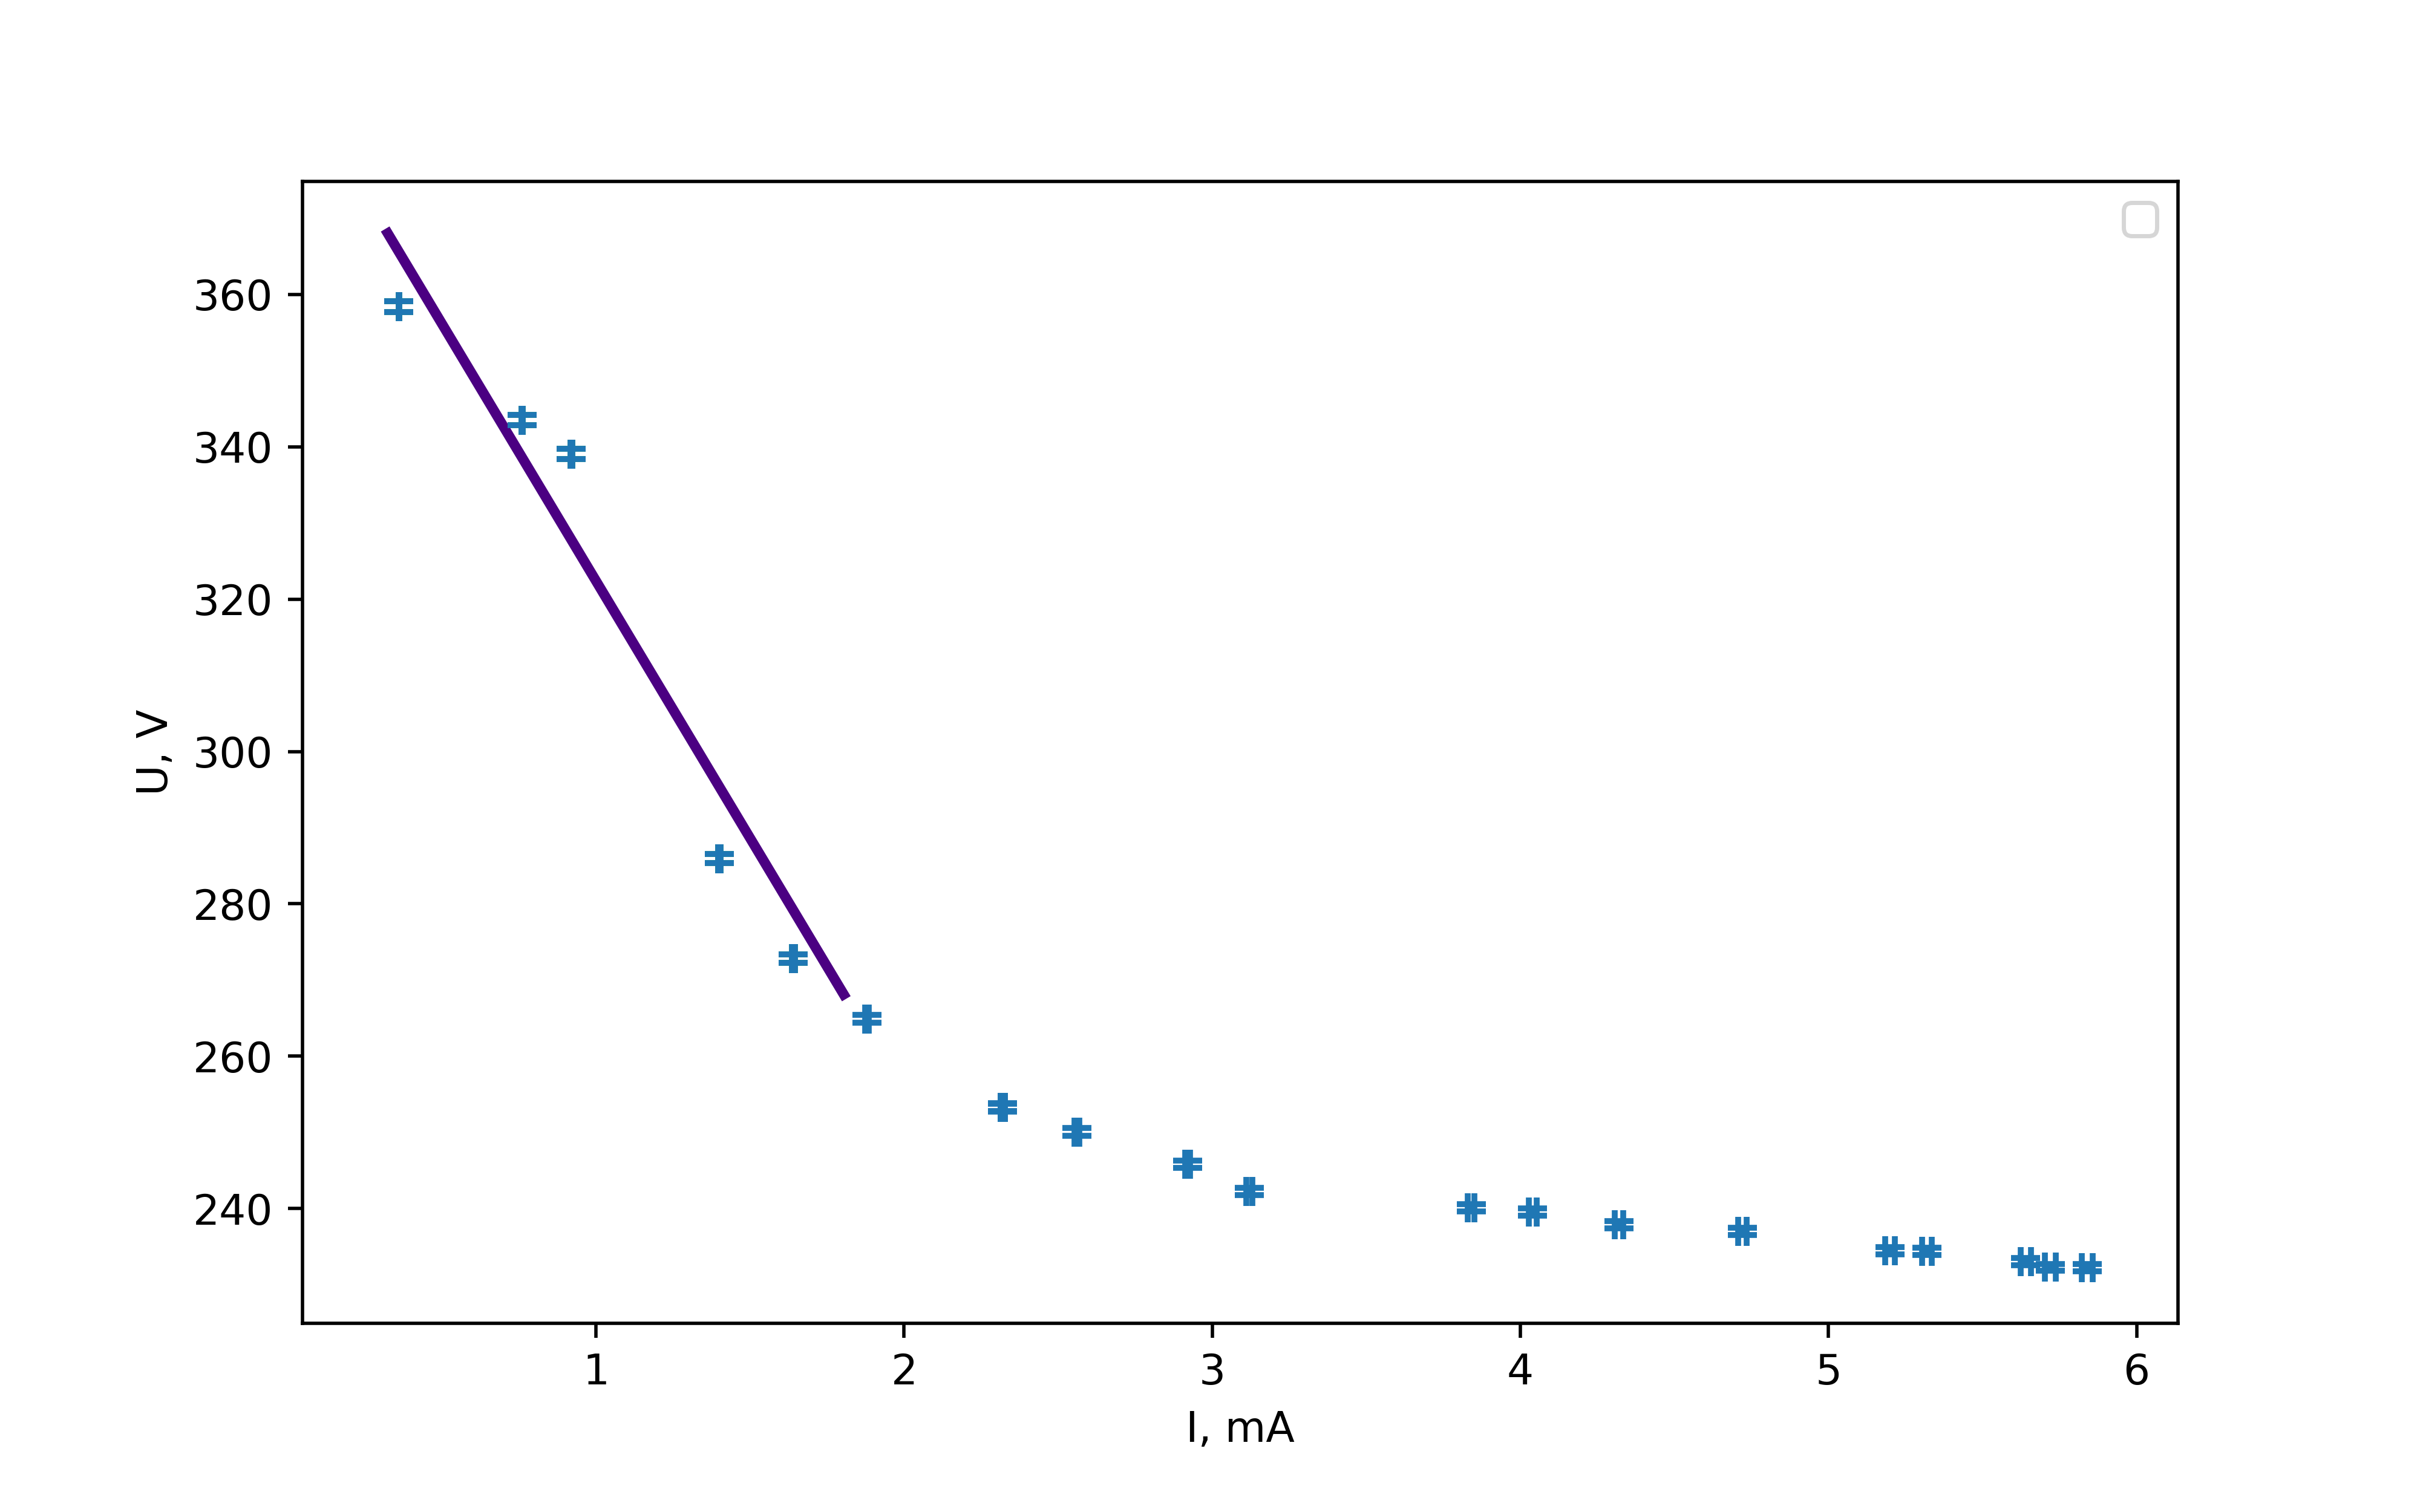
\includegraphics[width=\textwidth]{U(I)_discharge}
\caption{Вольт-амперная характеристика разряда в неоне при давлении $P \sim$ 2 торр, температуре ионов $T_i \approx $ 300 K.} \label{ВАХ_разряда}
\end{center}
\end{figure}

По наклону кривой определено максимальное $R_{диф}=\frac{dU}{dI} = -68 \pm 11$ кОм. Полученный участок вольт-амперной характеристики соответствует поднормальному тлеющему разряду.

\subsection{Зондовые характеристики} 
Для определения характеристик плазмы в неоне при фиксированном токе разряда измерена вольт-амперная характеристика двойного зонда. (рис. \ref{ВАХ_зонда}). Для каждой зондовой характеристики определен ионный ток и наклон характеристики в начале координат по графику. Из полученных результатов рассчитаны $T_e$, $n_i$, $\omega_p$, $r_{De}$, $r_D$, $N_D$, $\alpha$ - степень ионизации плазмы (по формулам из таблицы \ref{формулы}). Результаты приведены в таблице \ref{data}, также построены графики зависимости 
электронной температуры и концентрации электронов от тока разряда (рис. \ref{от_тока_разряда}).

\begin{figure}[h!]
\begin{center}
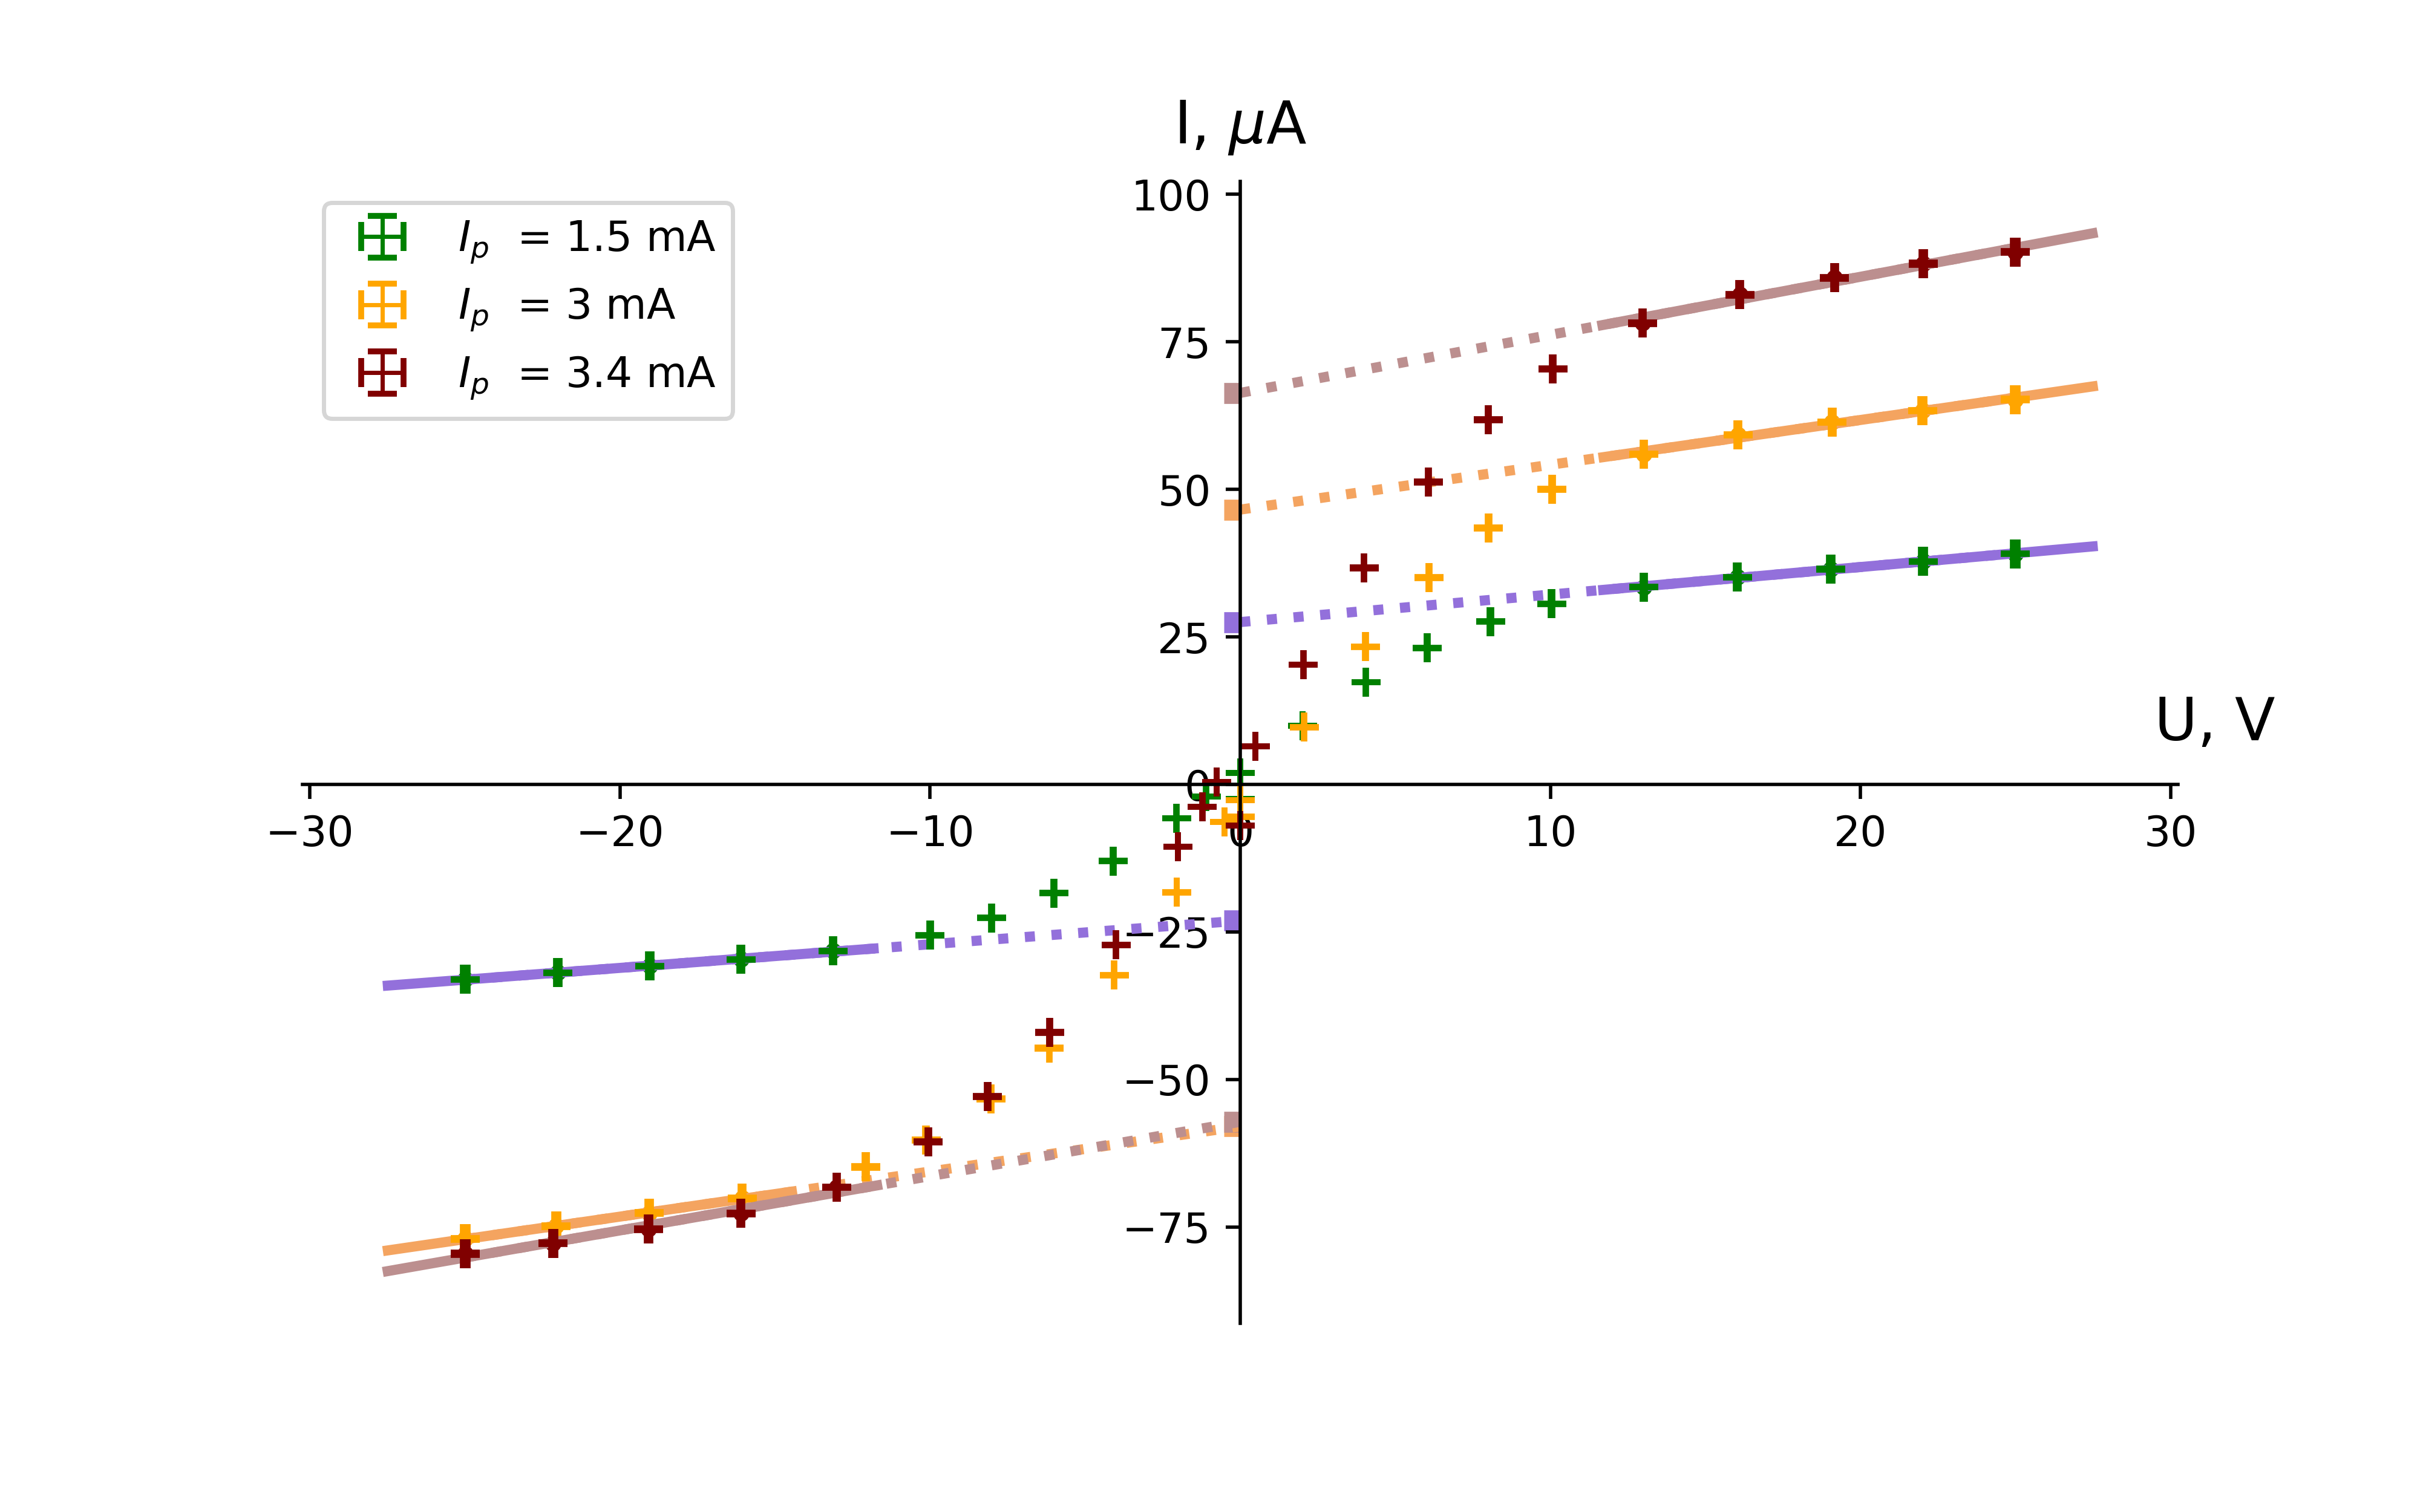
\includegraphics[width=\textwidth]{I(U)_probe}
\caption{Вольт-амперная характеристика двойного зонда при токах $\sim 50 \mu $ A, давлении $P \sim$ 2 торр, температуре ионов $T_i \approx $ 300 K.} \label{ВАХ_зонда}
\end{center}
\end{figure}

\begin{table}[h!]
\caption{Характеристики плазмы в неоне при давлении $P \sim$ 2 торр, температуре ионов $T_i \approx $ 300 K для разных токов разряда $I_p$}
\label{data}
\begin{tabular}{|l|l|l|l|}
\hline
$I_p,$ мА                & 1.5               & 3                 & 3.4               \\ \hline
$T_e,$ эВ                & $ 3.08 \pm 0.25 $   & $ 4.23 \pm 0.10 $   & $ 3.7 \pm 0.4 $   \\ \hline
$n_i, 10^{10}$ $ 1/см^3$    & $ 2.12 \pm 0.09 $   & $ 4.55 \pm 0.06 $   & $ 4.8 \pm 0.3 $   \\ \hline
$\omega_p, 10^{9}$ $ рад/с$ & $ 8.21 \pm 0.17 $   & $ 12.03 \pm 0.08 $  & $ 12.4 \pm 0.4 $  \\ \hline
$r_{De}, 10^{-3} $ $см$     & $ 9.0 \pm 0.8 $   & $ 7.17 \pm 0.20 $   & $ 6.5 \pm 0.7 $   \\ \hline
$r_{D}, 10^{-3} $ $см$      & $ 0.82 \pm 0.03 $ & $ 0.561 \pm 0.075 $ & $ 0.54 \pm 0.03 $ \\ \hline
$N_{D}$                  & $ 49 \pm 6 $      & $ 34 \pm 1 $      & $ 33 \pm 6 $      \\ \hline
$\alpha, 10^{-5}$        & $ 3.9 \pm 0.4 $   & $ 11.6 \pm 0.3 $  & $ 10.7 \pm 1.2 $  \\ \hline
\end{tabular}
\end{table}


\begin{figure}[h!]
\begin{center}
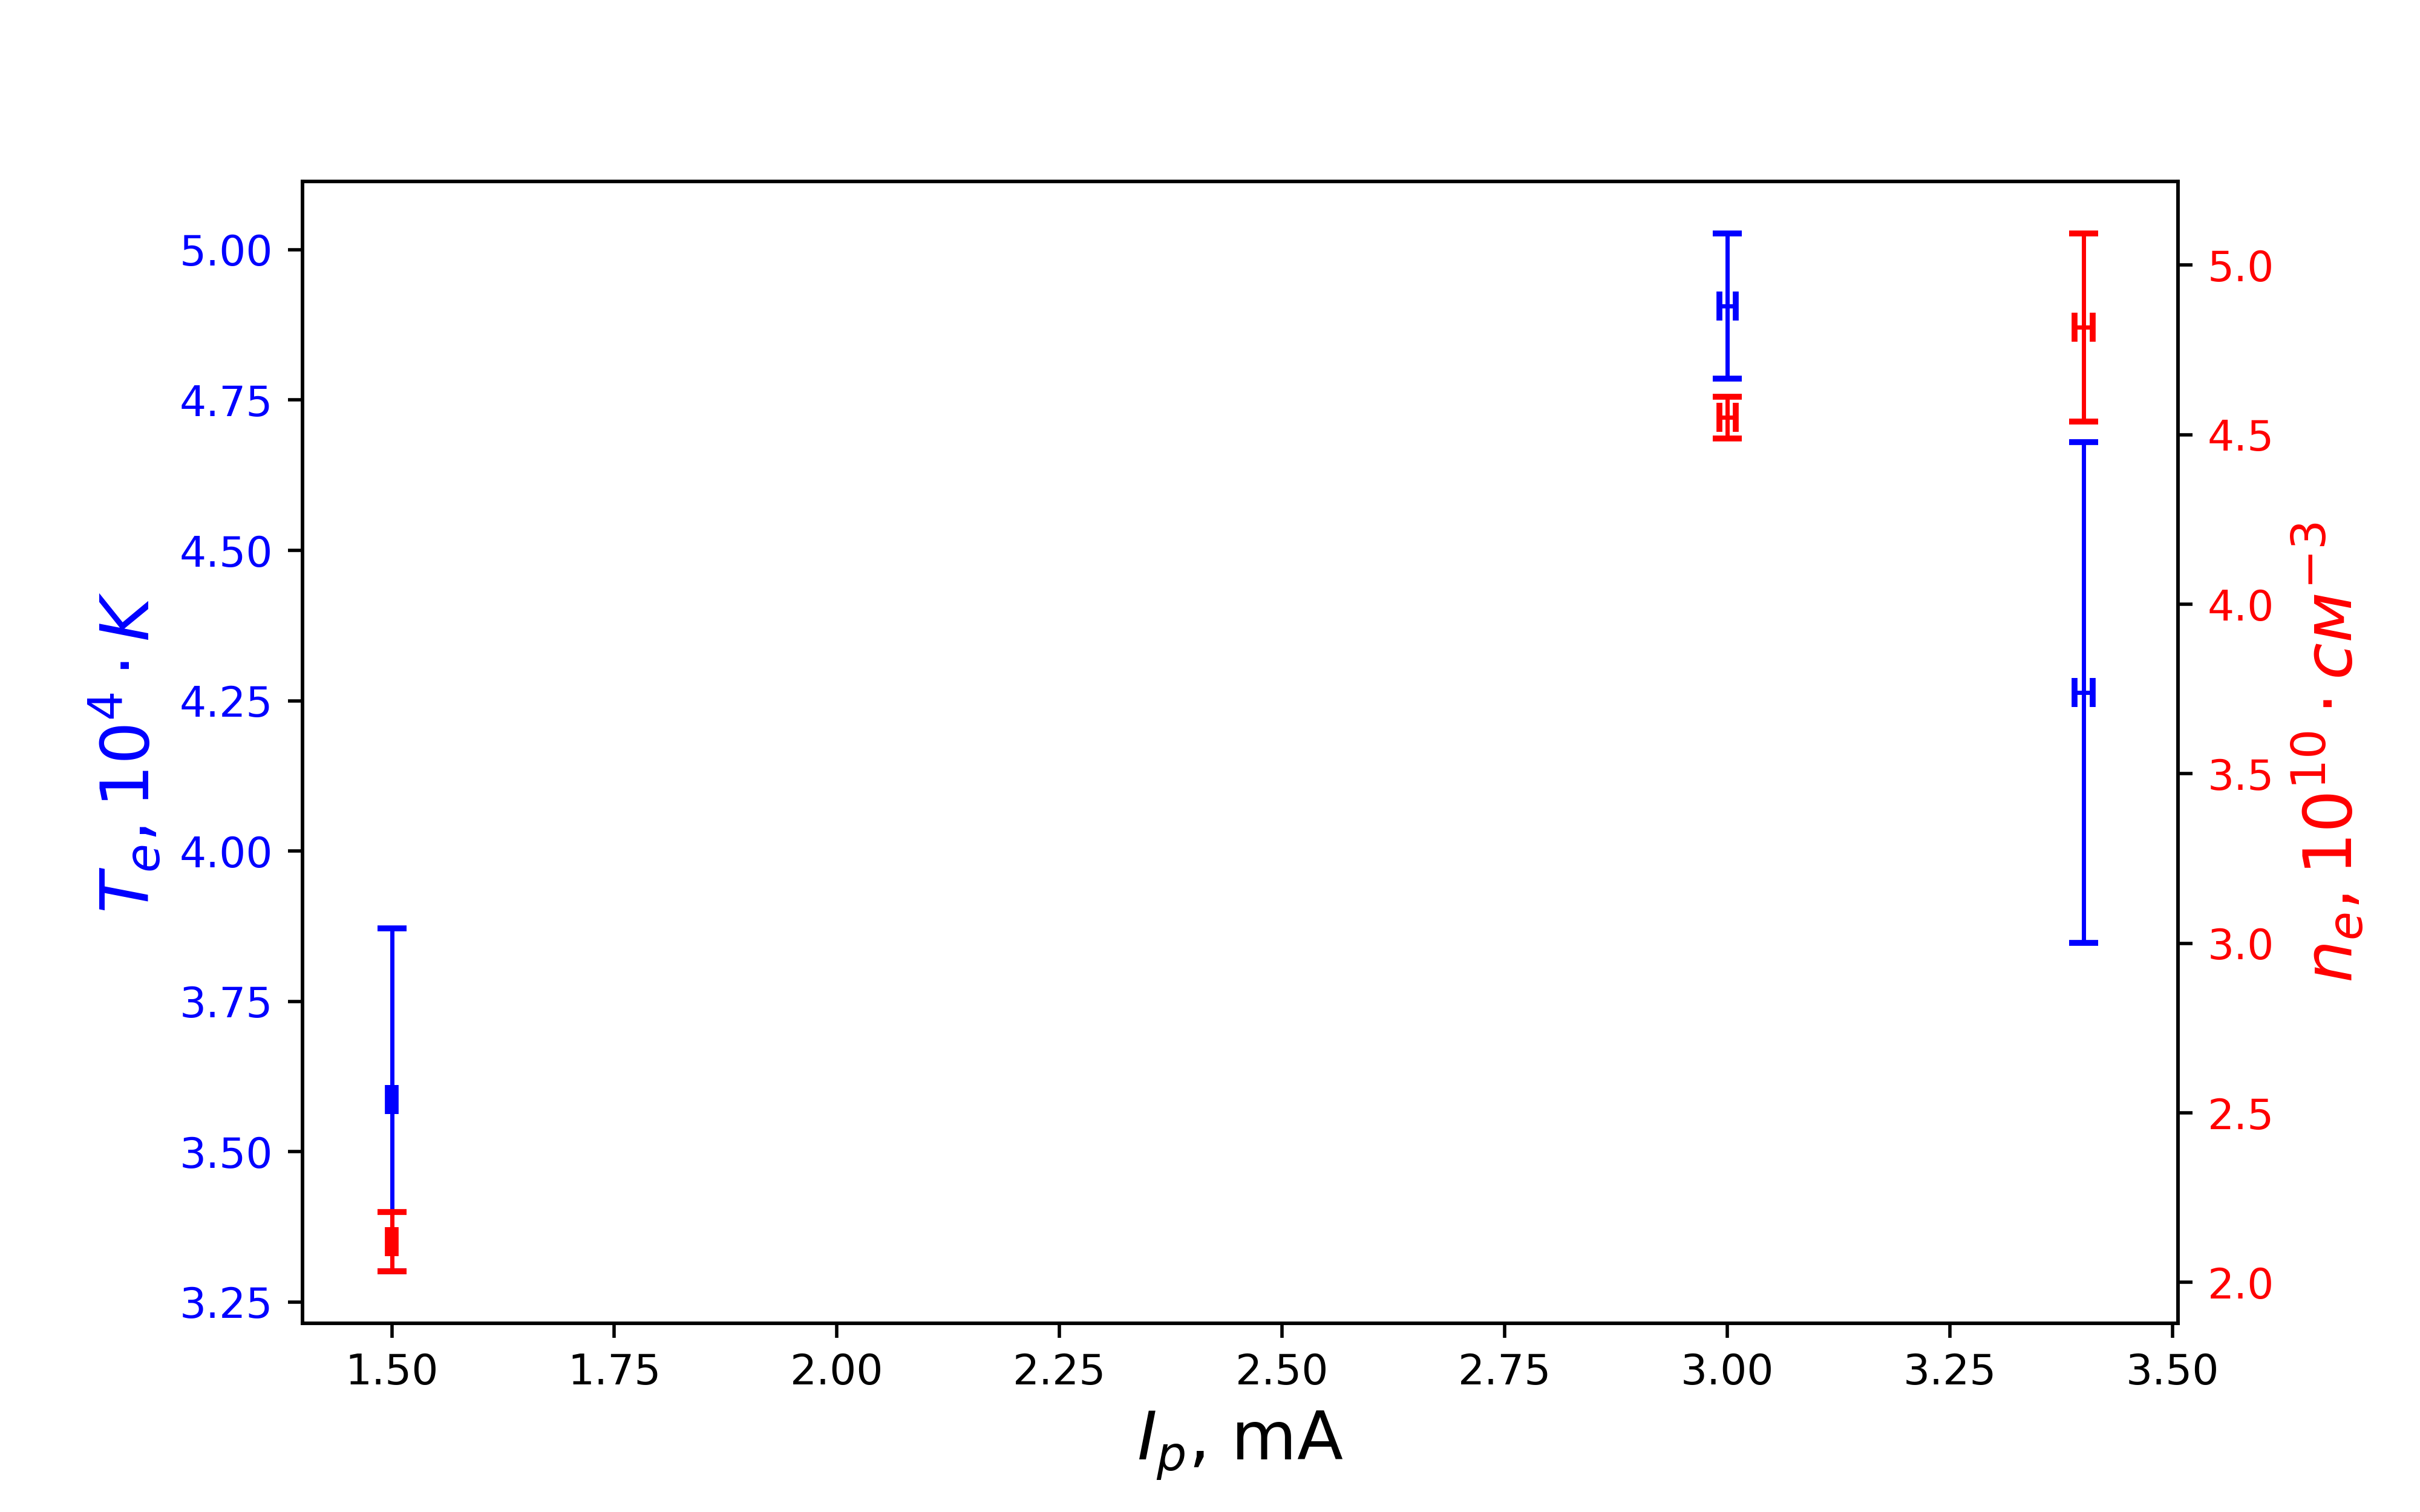
\includegraphics[width=\textwidth]{T,n(I_p)}
\caption{Зависимость электронной температуры и концентрации электронов от тока разряда в плазме неона при давлении $P \sim$ 2 торр, температуре ионов $T_i \approx $ 300 K.} \label{от_тока_разряда}
\end{center}
\end{figure}

\section{Обсуждение результатов}


1.  При сравнении вольт-амперной характеристики разряда (рис. \ref{ВАХ_разряда}) и графика вольт-амперной характеристики газового разряда из \cite{labnik} (рис. \ref{приложение}) видно, что рассматривался участок, соответствующий поднормальному тлеющему разряду.

\begin{figure}[h!]
\begin{center}
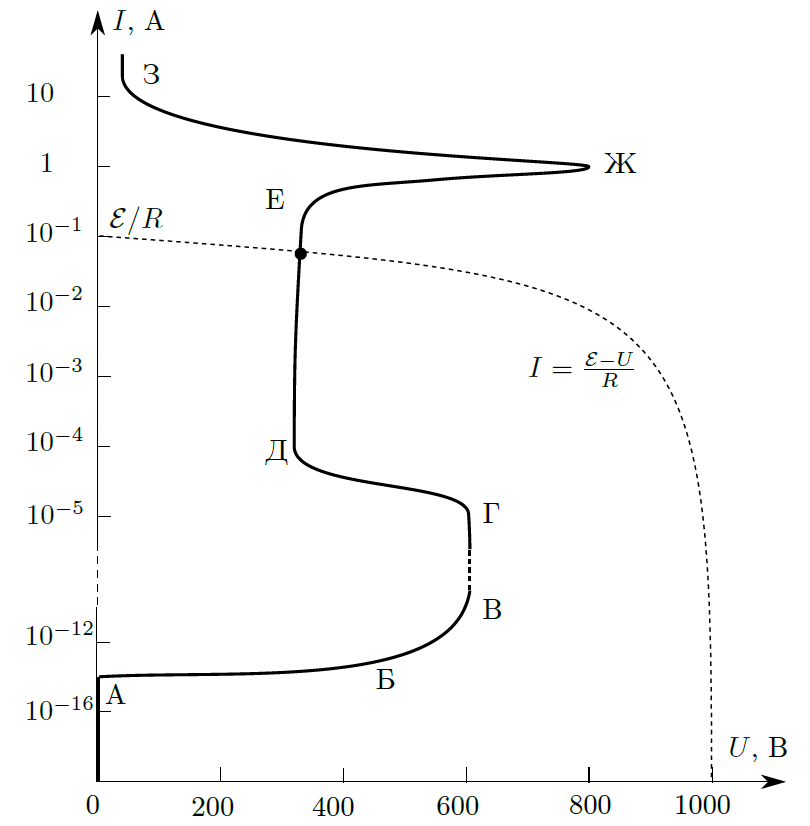
\includegraphics[width=0.5\textwidth]{Приложение}
\caption{Качественный вид вольт-амперной характеристики разряда в неоне при давлении $P \sim$ 1 торр (из \cite{labnik}). АБ - режим газового усилителя, ВГ - темный таунсендовский разряд, ГД - поднормальный тлеющий разряд, ДЕ - нормальный тлеющий разряд, ЕЖ - анормальный тлеющий разряд, ЖЗ - дуговой разряд} \label{приложение}
\end{center}
\end{figure}

2. По определению поляризационной длины $r_{De}$ плазму можно считать квазинейтральной, так как именно электронная дебаевская длина определяет масштаб, на котором нарушается квазинейтральность из-за тепловых флуктуаций электронов относительно ионов, а $r_{De} \sim 10^{-2} см$, что много меньше размеров области.

3. Оценив число ионов в дебаевской сфере $N_D \sim 40$, видно, что число частиц много больше 1, что позволяет называть плазму идеальной.

4. Определить зависимость электронной температуры от тока разряда с помощью полученных данных (рис. \ref{от_тока_разряда}) невозможно из-за малого числа точек и достаточной погрешности результатов. Однако можно качественно оценить зависимость концентрации электронов от тока разряда: график напоминает линейную или степенную зависимость, что достаточно ожидаемо, при увеличении тока разряда увеличивается и число электронов в газе.


\section{Выводы}
Из вольт-амперной характеристики разряда получено, что исследовался тлеющий газовый разряд. 
Экспериментальная зондовая характеристика схожа с теоретической зависимостью: $I = I_{iн} th\frac{eU}{2k_БT_e}$, количество ионов в дебаевской сфере $N_D \sim 40$ показывает идеальность плазмы. Остальные характеристики плазмы получились схожими с табличными значениями \cite{labnik}, что показало справедливость метода измерений. Однако не удалось оценить зависимость температуры электронов от тока разряда из-за неточных измерений и малого их числа.


\begin{thebibliography}{}
    \bibitem{labnik}  Никулин М.Г., Попов П.В., Нозик А.А. и др. Лабораторный практикум по общей физике : учеб. пособие. В трех томах. Т. 2. Электричество и магнетизм
\end{thebibliography}

\end{document}